\documentclass[1p]{elsarticle_modified}
%\bibliographystyle{elsarticle-num}

%\usepackage[colorlinks]{hyperref}
%\usepackage{abbrmath_seonhwa} %\Abb, \Ascr, \Acal ,\Abf, \Afrak
\usepackage{amsfonts}
\usepackage{amssymb}
\usepackage{amsmath}
\usepackage{amsthm}
\usepackage{scalefnt}
\usepackage{amsbsy}
\usepackage{kotex}
\usepackage{caption}
\usepackage{subfig}
\usepackage{color}
\usepackage{graphicx}
\usepackage{xcolor} %% white, black, red, green, blue, cyan, magenta, yellow
\usepackage{float}
\usepackage{setspace}
\usepackage{hyperref}

\usepackage{tikz}
\usetikzlibrary{arrows}

\usepackage{multirow}
\usepackage{array} % fixed length table
\usepackage{hhline}

%%%%%%%%%%%%%%%%%%%%%
\makeatletter
\renewcommand*\env@matrix[1][\arraystretch]{%
	\edef\arraystretch{#1}%
	\hskip -\arraycolsep
	\let\@ifnextchar\new@ifnextchar
	\array{*\c@MaxMatrixCols c}}
\makeatother %https://tex.stackexchange.com/questions/14071/how-can-i-increase-the-line-spacing-in-a-matrix
%%%%%%%%%%%%%%%

\usepackage[normalem]{ulem}

\newcommand{\msout}[1]{\ifmmode\text{\sout{\ensuremath{#1}}}\else\sout{#1}\fi}
%SOURCE: \msout is \stkout macro in https://tex.stackexchange.com/questions/20609/strikeout-in-math-mode

\newcommand{\cancel}[1]{
	\ifmmode
	{\color{red}\msout{#1}}
	\else
	{\color{red}\sout{#1}}
	\fi
}

\newcommand{\add}[1]{
	{\color{blue}\uwave{#1}}
}

\newcommand{\replace}[2]{
	\ifmmode
	{\color{red}\msout{#1}}{\color{blue}\uwave{#2}}
	\else
	{\color{red}\sout{#1}}{\color{blue}\uwave{#2}}
	\fi
}

\newcommand{\Sol}{\mathcal{S}} %segment
\newcommand{\D}{D} %diagram
\newcommand{\A}{\mathcal{A}} %arc


%%%%%%%%%%%%%%%%%%%%%%%%%%%%%5 test

\def\sl{\operatorname{\textup{SL}}(2,\Cbb)}
\def\psl{\operatorname{\textup{PSL}}(2,\Cbb)}
\def\quan{\mkern 1mu \triangleright \mkern 1mu}

\theoremstyle{definition}
\newtheorem{thm}{Theorem}[section]
\newtheorem{prop}[thm]{Proposition}
\newtheorem{lem}[thm]{Lemma}
\newtheorem{ques}[thm]{Question}
\newtheorem{cor}[thm]{Corollary}
\newtheorem{defn}[thm]{Definition}
\newtheorem{exam}[thm]{Example}
\newtheorem{rmk}[thm]{Remark}
\newtheorem{alg}[thm]{Algorithm}

\newcommand{\I}{\sqrt{-1}}
\begin{document}

%\begin{frontmatter}
%
%\title{Boundary parabolic representations of knots up to 8 crossings}
%
%%% Group authors per affiliation:
%\author{Yunhi Cho} 
%\address{Department of Mathematics, University of Seoul, Seoul, Korea}
%\ead{yhcho@uos.ac.kr}
%
%
%\author{Seonhwa Kim} %\fnref{s_kim}}
%\address{Center for Geometry and Physics, Institute for Basic Science, Pohang, 37673, Korea}
%\ead{ryeona17@ibs.re.kr}
%
%\author{Hyuk Kim}
%\address{Department of Mathematical Sciences, Seoul National University, Seoul 08826, Korea}
%\ead{hyukkim@snu.ac.kr}
%
%\author{Seokbeom Yoon}
%\address{Department of Mathematical Sciences, Seoul National University, Seoul, 08826,  Korea}
%\ead{sbyoon15@snu.ac.kr}
%
%\begin{abstract}
%We find all boundary parabolic representation of knots up to 8 crossings.
%
%\end{abstract}
%\begin{keyword}
%    \MSC[2010] 57M25 
%\end{keyword}
%
%\end{frontmatter}

%\linenumbers
%\tableofcontents
%
\newcommand\colored[1]{\textcolor{white}{\rule[-0.35ex]{0.8em}{1.4ex}}\kern-0.8em\color{red} #1}%
%\newcommand\colored[1]{\textcolor{white}{ #1}\kern-2.17ex	\textcolor{white}{ #1}\kern-1.81ex	\textcolor{white}{ #1}\kern-2.15ex\color{red}#1	}

{\Large $\underline{12a_{0514}~(K12a_{0514})}$}

\setlength{\tabcolsep}{10pt}
\renewcommand{\arraystretch}{1.6}
\vspace{1cm}\begin{tabular}{m{100pt}>{\centering\arraybackslash}m{274pt}}
\multirow{5}{120pt}{
	\centering
	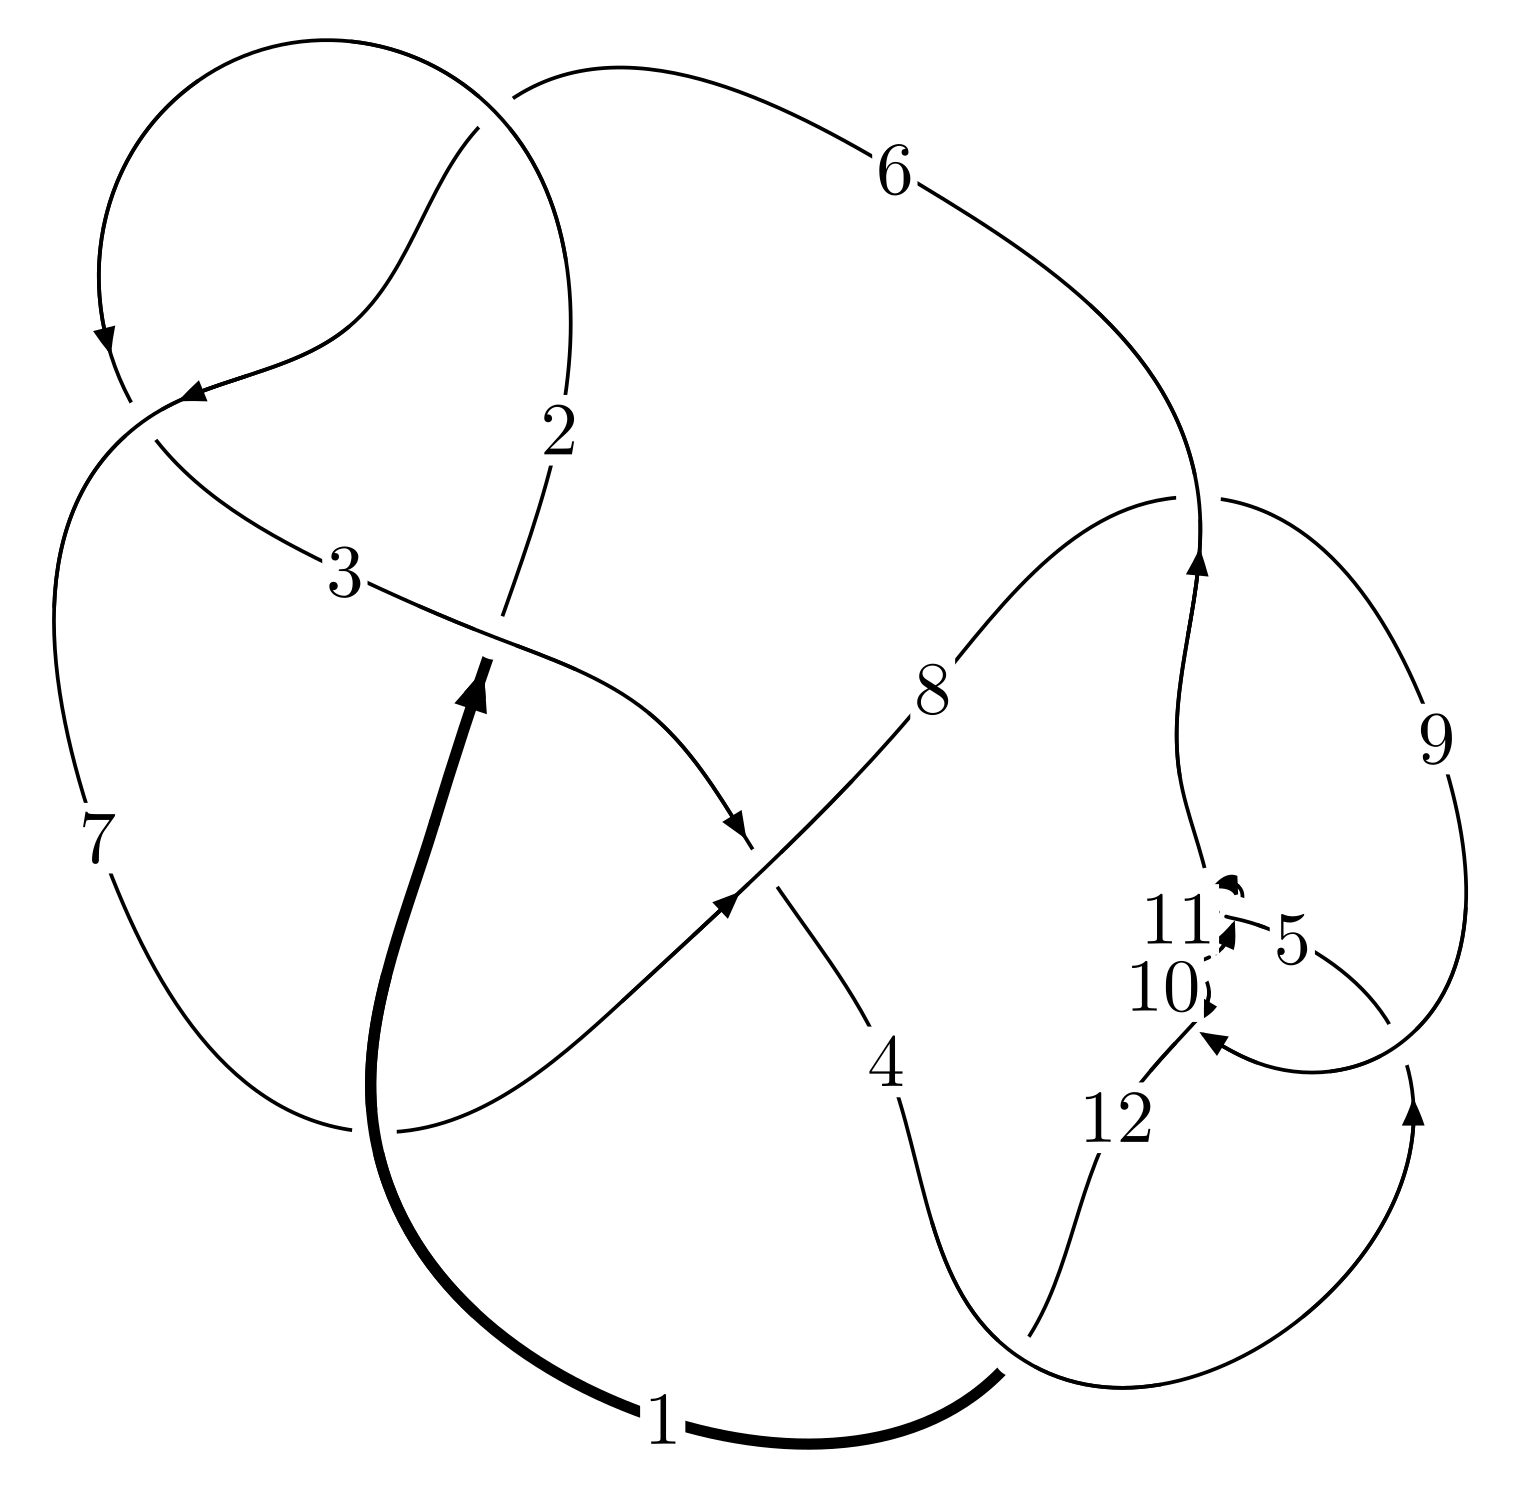
\includegraphics[width=112pt]{../../../GIT/diagram.site/Diagrams/png/1315_12a_0514.png}\\
\ \ \ A knot diagram\footnotemark}&
\allowdisplaybreaks
\textbf{Linearized knot diagam} \\
\cline{2-2}
 &
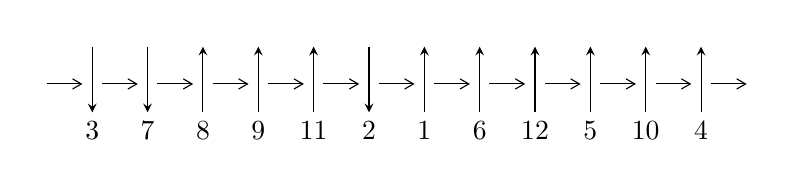
\begin{tikzpicture}[x=20pt, y=17pt]
	% nodes
	\node (C0) at (0, 0) {};
	\node (C1) at (1, 0) {};
	\node (C1U) at (1, +1) {};
	\node (C1D) at (1, -1) {3};

	\node (C2) at (2, 0) {};
	\node (C2U) at (2, +1) {};
	\node (C2D) at (2, -1) {7};

	\node (C3) at (3, 0) {};
	\node (C3U) at (3, +1) {};
	\node (C3D) at (3, -1) {8};

	\node (C4) at (4, 0) {};
	\node (C4U) at (4, +1) {};
	\node (C4D) at (4, -1) {9};

	\node (C5) at (5, 0) {};
	\node (C5U) at (5, +1) {};
	\node (C5D) at (5, -1) {11};

	\node (C6) at (6, 0) {};
	\node (C6U) at (6, +1) {};
	\node (C6D) at (6, -1) {2};

	\node (C7) at (7, 0) {};
	\node (C7U) at (7, +1) {};
	\node (C7D) at (7, -1) {1};

	\node (C8) at (8, 0) {};
	\node (C8U) at (8, +1) {};
	\node (C8D) at (8, -1) {6};

	\node (C9) at (9, 0) {};
	\node (C9U) at (9, +1) {};
	\node (C9D) at (9, -1) {12};

	\node (C10) at (10, 0) {};
	\node (C10U) at (10, +1) {};
	\node (C10D) at (10, -1) {5};

	\node (C11) at (11, 0) {};
	\node (C11U) at (11, +1) {};
	\node (C11D) at (11, -1) {10};

	\node (C12) at (12, 0) {};
	\node (C12U) at (12, +1) {};
	\node (C12D) at (12, -1) {4};
	\node (C13) at (13, 0) {};

	% arrows
	\draw[->,>={angle 60}]
	(C0) edge (C1) (C1) edge (C2) (C2) edge (C3) (C3) edge (C4) (C4) edge (C5) (C5) edge (C6) (C6) edge (C7) (C7) edge (C8) (C8) edge (C9) (C9) edge (C10) (C10) edge (C11) (C11) edge (C12) (C12) edge (C13) ;	\draw[->,>=stealth]
	(C1U) edge (C1D) (C2U) edge (C2D) (C3D) edge (C3U) (C4D) edge (C4U) (C5D) edge (C5U) (C6U) edge (C6D) (C7D) edge (C7U) (C8D) edge (C8U) (C9D) edge (C9U) (C10D) edge (C10U) (C11D) edge (C11U) (C12D) edge (C12U) ;
	\end{tikzpicture} \\
\hhline{~~} \\& 
\textbf{Solving Sequence} \\ \cline{2-2} 
 &
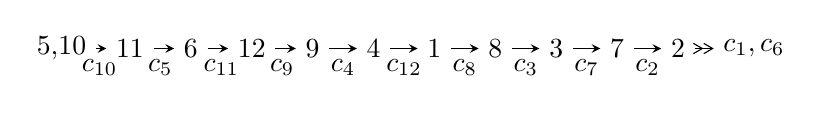
\begin{tikzpicture}[x=22pt, y=7pt]
	% node
	\node (A0) at (-1/8, 0) {5,10};
	\node (A1) at (1, 0) {11};
	\node (A2) at (2, 0) {6};
	\node (A3) at (3, 0) {12};
	\node (A4) at (4, 0) {9};
	\node (A5) at (5, 0) {4};
	\node (A6) at (6, 0) {1};
	\node (A7) at (7, 0) {8};
	\node (A8) at (8, 0) {3};
	\node (A9) at (9, 0) {7};
	\node (A10) at (10, 0) {2};
	\node (C1) at (1/2, -1) {$c_{10}$};
	\node (C2) at (3/2, -1) {$c_{5}$};
	\node (C3) at (5/2, -1) {$c_{11}$};
	\node (C4) at (7/2, -1) {$c_{9}$};
	\node (C5) at (9/2, -1) {$c_{4}$};
	\node (C6) at (11/2, -1) {$c_{12}$};
	\node (C7) at (13/2, -1) {$c_{8}$};
	\node (C8) at (15/2, -1) {$c_{3}$};
	\node (C9) at (17/2, -1) {$c_{7}$};
	\node (C10) at (19/2, -1) {$c_{2}$};
	\node (A11) at (45/4, 0) {$c_{1},c_{6}$};

	% edge
	\draw[->,>=stealth]	
	(A0) edge (A1) (A1) edge (A2) (A2) edge (A3) (A3) edge (A4) (A4) edge (A5) (A5) edge (A6) (A6) edge (A7) (A7) edge (A8) (A8) edge (A9) (A9) edge (A10) ;
	\draw[->>,>={angle 60}]	
	(A10) edge (A11);
\end{tikzpicture} \\ 

\end{tabular} \\

\footnotetext{
The image of knot diagram is generated by the software ``\textbf{Draw programme}" developed by Andrew Bartholomew(\url{http://www.layer8.co.uk/maths/draw/index.htm\#Running-draw}), where we modified some parts for our purpose(\url{https://github.com/CATsTAILs/LinksPainter}).
}\phantom \\ \newline 
\centering \textbf{Ideals for irreducible components\footnotemark of $X_{\text{par}}$} 
 
\begin{align*}
I^u_{1}&=\langle 
u^{93}- u^{92}+\cdots- u+1\rangle \\
\\
\end{align*}
\raggedright * 1 irreducible components of $\dim_{\mathbb{C}}=0$, with total 93 representations.\\
\footnotetext{All coefficients of polynomials are rational numbers. But the coefficients are sometimes approximated in decimal forms when there is not enough margin.}
\newpage
\renewcommand{\arraystretch}{1}
\centering \section*{I. $I^u_{1}= \langle u^{93}- u^{92}+\cdots- u+1 \rangle$}
\flushleft \textbf{(i) Arc colorings}\\
\begin{tabular}{m{7pt} m{180pt} m{7pt} m{180pt} }
\flushright $a_{5}=$&$\begin{pmatrix}0\\u\end{pmatrix}$ \\
\flushright $a_{10}=$&$\begin{pmatrix}1\\0\end{pmatrix}$ \\
\flushright $a_{11}=$&$\begin{pmatrix}1\\- u^2\end{pmatrix}$ \\
\flushright $a_{6}=$&$\begin{pmatrix}u\\- u^3+u\end{pmatrix}$ \\
\flushright $a_{12}=$&$\begin{pmatrix}- u^2+1\\- u^2\end{pmatrix}$ \\
\flushright $a_{9}=$&$\begin{pmatrix}u^4- u^2+1\\u^4\end{pmatrix}$ \\
\flushright $a_{4}=$&$\begin{pmatrix}- u^9+2 u^7-3 u^5+2 u^3- u\\- u^9+u^7- u^5+u\end{pmatrix}$ \\
\flushright $a_{1}=$&$\begin{pmatrix}- u^{16}+3 u^{14}-7 u^{12}+10 u^{10}-11 u^8+8 u^6-4 u^4+1\\- u^{16}+2 u^{14}-4 u^{12}+4 u^{10}-2 u^8+2 u^4-2 u^2\end{pmatrix}$ \\
\flushright $a_{8}=$&$\begin{pmatrix}- u^8+u^6- u^4+1\\u^{10}-2 u^8+3 u^6-2 u^4+u^2\end{pmatrix}$ \\
\flushright $a_{3}=$&$\begin{pmatrix}u^{27}-4 u^{25}+\cdots+u^3-2 u\\- u^{29}+5 u^{27}+\cdots- u^3+u\end{pmatrix}$ \\
\flushright $a_{7}=$&$\begin{pmatrix}- u^{42}+7 u^{40}+\cdots-3 u^2+1\\- u^{42}+6 u^{40}+\cdots+4 u^4+u^2\end{pmatrix}$ \\
\flushright $a_{2}=$&$\begin{pmatrix}u^{72}-11 u^{70}+\cdots-2 u^2+1\\- u^{74}+12 u^{72}+\cdots-4 u^4- u^2\end{pmatrix}$\\&\end{tabular}
\flushleft \textbf{(ii) Obstruction class $= -1$}\\~\\
\flushleft \textbf{(iii) Cusp Shapes $= -4 u^{91}+56 u^{89}+\cdots-12 u+2$}\\~\\
\newpage\renewcommand{\arraystretch}{1}
\flushleft \textbf{(iv) u-Polynomials at the component}\newline \\
\begin{tabular}{m{50pt}|m{274pt}}
Crossings & \hspace{64pt}u-Polynomials at each crossing \\
\hline $$\begin{aligned}c_{1}\end{aligned}$$&$\begin{aligned}
&u^{93}+45 u^{92}+\cdots+3 u+1
\end{aligned}$\\
\hline $$\begin{aligned}c_{2},c_{6}\end{aligned}$$&$\begin{aligned}
&u^{93}- u^{92}+\cdots+3 u-1
\end{aligned}$\\
\hline $$\begin{aligned}c_{3}\end{aligned}$$&$\begin{aligned}
&u^{93}+u^{92}+\cdots-15 u-1
\end{aligned}$\\
\hline $$\begin{aligned}c_{4}\end{aligned}$$&$\begin{aligned}
&u^{93}- u^{92}+\cdots+3237 u-481
\end{aligned}$\\
\hline $$\begin{aligned}c_{5},c_{10}\end{aligned}$$&$\begin{aligned}
&u^{93}+u^{92}+\cdots- u-1
\end{aligned}$\\
\hline $$\begin{aligned}c_{7}\end{aligned}$$&$\begin{aligned}
&u^{93}-3 u^{92}+\cdots+6347 u-949
\end{aligned}$\\
\hline $$\begin{aligned}c_{8},c_{12}\end{aligned}$$&$\begin{aligned}
&u^{93}+7 u^{92}+\cdots+9 u+5
\end{aligned}$\\
\hline $$\begin{aligned}c_{9},c_{11}\end{aligned}$$&$\begin{aligned}
&u^{93}-29 u^{92}+\cdots+3 u-1
\end{aligned}$\\
\hline
\end{tabular}\\~\\
\newpage\renewcommand{\arraystretch}{1}
\flushleft \textbf{(v) Riley Polynomials at the component}\newline \\
\begin{tabular}{m{50pt}|m{274pt}}
Crossings & \hspace{64pt}Riley Polynomials at each crossing \\
\hline $$\begin{aligned}c_{1}\end{aligned}$$&$\begin{aligned}
&y^{93}+7 y^{92}+\cdots-9 y-1
\end{aligned}$\\
\hline $$\begin{aligned}c_{2},c_{6}\end{aligned}$$&$\begin{aligned}
&y^{93}-45 y^{92}+\cdots+3 y-1
\end{aligned}$\\
\hline $$\begin{aligned}c_{3}\end{aligned}$$&$\begin{aligned}
&y^{93}+3 y^{92}+\cdots-61 y-1
\end{aligned}$\\
\hline $$\begin{aligned}c_{4}\end{aligned}$$&$\begin{aligned}
&y^{93}+23 y^{92}+\cdots-5811377 y-231361
\end{aligned}$\\
\hline $$\begin{aligned}c_{5},c_{10}\end{aligned}$$&$\begin{aligned}
&y^{93}-29 y^{92}+\cdots+3 y-1
\end{aligned}$\\
\hline $$\begin{aligned}c_{7}\end{aligned}$$&$\begin{aligned}
&y^{93}+31 y^{92}+\cdots-22453981 y-900601
\end{aligned}$\\
\hline $$\begin{aligned}c_{8},c_{12}\end{aligned}$$&$\begin{aligned}
&y^{93}+75 y^{92}+\cdots-1129 y-25
\end{aligned}$\\
\hline $$\begin{aligned}c_{9},c_{11}\end{aligned}$$&$\begin{aligned}
&y^{93}+71 y^{92}+\cdots+7 y-1
\end{aligned}$\\
\hline
\end{tabular}\\~\\
\newpage\flushleft \textbf{(vi) Complex Volumes and Cusp Shapes}
$$\begin{array}{c|c|c}  
\text{Solutions to }I^u_{1}& \I (\text{vol} + \sqrt{-1}CS) & \text{Cusp shape}\\
 \hline 
\begin{aligned}
u &= \phantom{-}1.001330 + 0.020624 I\end{aligned}
 & \phantom{-}5.22907 + 0.91927 I & \phantom{-0.000000 } 0 \\ \hline\begin{aligned}
u &= \phantom{-}1.001330 - 0.020624 I\end{aligned}
 & \phantom{-}5.22907 - 0.91927 I & \phantom{-0.000000 } 0 \\ \hline\begin{aligned}
u &= \phantom{-}0.950842 + 0.299864 I\end{aligned}
 & -2.51592 - 5.16810 I & \phantom{-0.000000 } 0 \\ \hline\begin{aligned}
u &= \phantom{-}0.950842 - 0.299864 I\end{aligned}
 & -2.51592 + 5.16810 I & \phantom{-0.000000 } 0 \\ \hline\begin{aligned}
u &= \phantom{-}0.971710 + 0.262556 I\end{aligned}
 & -4.09655 + 2.66309 I & \phantom{-0.000000 } 0 \\ \hline\begin{aligned}
u &= \phantom{-}0.971710 - 0.262556 I\end{aligned}
 & -4.09655 - 2.66309 I & \phantom{-0.000000 } 0 \\ \hline\begin{aligned}
u &= -1.010030 + 0.039683 I\end{aligned}
 & \phantom{-}3.45576 - 5.61543 I & \phantom{-0.000000 } 0 \\ \hline\begin{aligned}
u &= -1.010030 - 0.039683 I\end{aligned}
 & \phantom{-}3.45576 + 5.61543 I & \phantom{-0.000000 } 0 \\ \hline\begin{aligned}
u &= \phantom{-}1.000590 + 0.171975 I\end{aligned}
 & \phantom{-}2.41507 + 4.46350 I & \phantom{-0.000000 } 0 \\ \hline\begin{aligned}
u &= \phantom{-}1.000590 - 0.171975 I\end{aligned}
 & \phantom{-}2.41507 - 4.46350 I & \phantom{-0.000000 } 0 \\ \hline\begin{aligned}
u &= -0.974861 + 0.137746 I\end{aligned}
 & \phantom{-}1.78185 - 0.05525 I & \phantom{-0.000000 } 0 \\ \hline\begin{aligned}
u &= -0.974861 - 0.137746 I\end{aligned}
 & \phantom{-}1.78185 + 0.05525 I & \phantom{-0.000000 } 0 \\ \hline\begin{aligned}
u &= \phantom{-}0.852921 + 0.560937 I\end{aligned}
 & -0.31851 + 4.89376 I & \phantom{-0.000000 } 0 \\ \hline\begin{aligned}
u &= \phantom{-}0.852921 - 0.560937 I\end{aligned}
 & -0.31851 - 4.89376 I & \phantom{-0.000000 } 0 \\ \hline\begin{aligned}
u &= -0.933380 + 0.277710 I\end{aligned}
 & -0.033888 + 0.415540 I & \phantom{-0.000000 } 0 \\ \hline\begin{aligned}
u &= -0.933380 - 0.277710 I\end{aligned}
 & -0.033888 - 0.415540 I & \phantom{-0.000000 } 0 \\ \hline\begin{aligned}
u &= \phantom{-}0.746143 + 0.706717 I\end{aligned}
 & -3.63252 + 0.94988 I & \phantom{-0.000000 } 0 \\ \hline\begin{aligned}
u &= \phantom{-}0.746143 - 0.706717 I\end{aligned}
 & -3.63252 - 0.94988 I & \phantom{-0.000000 } 0 \\ \hline\begin{aligned}
u &= -1.016430 + 0.215896 I\end{aligned}
 & -3.70029 - 3.19651 I & \phantom{-0.000000 } 0 \\ \hline\begin{aligned}
u &= -1.016430 - 0.215896 I\end{aligned}
 & -3.70029 + 3.19651 I & \phantom{-0.000000 } 0 \\ \hline\begin{aligned}
u &= \phantom{-}1.023660 + 0.199077 I\end{aligned}
 & \phantom{-}0.67170 + 6.17554 I & \phantom{-0.000000 } 0 \\ \hline\begin{aligned}
u &= \phantom{-}1.023660 - 0.199077 I\end{aligned}
 & \phantom{-}0.67170 - 6.17554 I & \phantom{-0.000000 } 0 \\ \hline\begin{aligned}
u &= \phantom{-}0.670081 + 0.679818 I\end{aligned}
 & -1.70281 - 5.79619 I & \phantom{-0.000000 } 0 \\ \hline\begin{aligned}
u &= \phantom{-}0.670081 - 0.679818 I\end{aligned}
 & -1.70281 + 5.79619 I & \phantom{-0.000000 } 0 \\ \hline\begin{aligned}
u &= -0.771220 + 0.558683 I\end{aligned}
 & \phantom{-}0.994657 - 0.499555 I & \phantom{-0.000000 } 0 \\ \hline\begin{aligned}
u &= -0.771220 - 0.558683 I\end{aligned}
 & \phantom{-}0.994657 + 0.499555 I & \phantom{-0.000000 } 0 \\ \hline\begin{aligned}
u &= -1.032350 + 0.202863 I\end{aligned}
 & -1.78029 - 11.11130 I & \phantom{-0.000000 } 0 \\ \hline\begin{aligned}
u &= -1.032350 - 0.202863 I\end{aligned}
 & -1.78029 + 11.11130 I & \phantom{-0.000000 } 0 \\ \hline\begin{aligned}
u &= -0.689312 + 0.649627 I\end{aligned}
 & \phantom{-}0.342510 + 1.086330 I & \phantom{-0.000000 } 0 \\ \hline\begin{aligned}
u &= -0.689312 - 0.649627 I\end{aligned}
 & \phantom{-}0.342510 - 1.086330 I & \phantom{-0.000000 } 0\\
 \hline 
 \end{array}$$\newpage$$\begin{array}{c|c|c}  
\text{Solutions to }I^u_{1}& \I (\text{vol} + \sqrt{-1}CS) & \text{Cusp shape}\\
 \hline 
\begin{aligned}
u &= -0.727491 + 0.813517 I\end{aligned}
 & -4.08031 + 3.83714 I & \phantom{-0.000000 } 0 \\ \hline\begin{aligned}
u &= -0.727491 - 0.813517 I\end{aligned}
 & -4.08031 - 3.83714 I & \phantom{-0.000000 } 0 \\ \hline\begin{aligned}
u &= \phantom{-}0.740790 + 0.801851 I\end{aligned}
 & -4.40160 + 0.77019 I & \phantom{-0.000000 } 0 \\ \hline\begin{aligned}
u &= \phantom{-}0.740790 - 0.801851 I\end{aligned}
 & -4.40160 - 0.77019 I & \phantom{-0.000000 } 0 \\ \hline\begin{aligned}
u &= -0.724420 + 0.831405 I\end{aligned}
 & -6.13241 + 5.62657 I & \phantom{-0.000000 } 0 \\ \hline\begin{aligned}
u &= -0.724420 - 0.831405 I\end{aligned}
 & -6.13241 - 5.62657 I & \phantom{-0.000000 } 0 \\ \hline\begin{aligned}
u &= \phantom{-}0.722484 + 0.835791 I\end{aligned}
 & -8.65339 - 10.61050 I & \phantom{-0.000000 } 0 \\ \hline\begin{aligned}
u &= \phantom{-}0.722484 - 0.835791 I\end{aligned}
 & -8.65339 + 10.61050 I & \phantom{-0.000000 } 0 \\ \hline\begin{aligned}
u &= \phantom{-}0.732247 + 0.834353 I\end{aligned}
 & -10.58940 - 2.51762 I & \phantom{-0.000000 } 0 \\ \hline\begin{aligned}
u &= \phantom{-}0.732247 - 0.834353 I\end{aligned}
 & -10.58940 + 2.51762 I & \phantom{-0.000000 } 0 \\ \hline\begin{aligned}
u &= \phantom{-}0.763399 + 0.821833 I\end{aligned}
 & -6.84470 + 1.82953 I & \phantom{-0.000000 } 0 \\ \hline\begin{aligned}
u &= \phantom{-}0.763399 - 0.821833 I\end{aligned}
 & -6.84470 - 1.82953 I & \phantom{-0.000000 } 0 \\ \hline\begin{aligned}
u &= \phantom{-}0.867613 + 0.712408 I\end{aligned}
 & -2.70656 + 2.72583 I & \phantom{-0.000000 } 0 \\ \hline\begin{aligned}
u &= \phantom{-}0.867613 - 0.712408 I\end{aligned}
 & -2.70656 - 2.72583 I & \phantom{-0.000000 } 0 \\ \hline\begin{aligned}
u &= -0.756825 + 0.829646 I\end{aligned}
 & -11.03530 + 1.47379 I & \phantom{-0.000000 } 0 \\ \hline\begin{aligned}
u &= -0.756825 - 0.829646 I\end{aligned}
 & -11.03530 - 1.47379 I & \phantom{-0.000000 } 0 \\ \hline\begin{aligned}
u &= -0.849545 + 0.742275 I\end{aligned}
 & -5.61738 + 0.89934 I & \phantom{-0.000000 } 0 \\ \hline\begin{aligned}
u &= -0.849545 - 0.742275 I\end{aligned}
 & -5.61738 - 0.89934 I & \phantom{-0.000000 } 0 \\ \hline\begin{aligned}
u &= -0.768568 + 0.826375 I\end{aligned}
 & -9.48988 - 6.65080 I & \phantom{-0.000000 } 0 \\ \hline\begin{aligned}
u &= -0.768568 - 0.826375 I\end{aligned}
 & -9.48988 + 6.65080 I & \phantom{-0.000000 } 0 \\ \hline\begin{aligned}
u &= \phantom{-}0.941591 + 0.622723 I\end{aligned}
 & \phantom{-}0.133887 - 0.249972 I & \phantom{-0.000000 } 0 \\ \hline\begin{aligned}
u &= \phantom{-}0.941591 - 0.622723 I\end{aligned}
 & \phantom{-}0.133887 + 0.249972 I & \phantom{-0.000000 } 0 \\ \hline\begin{aligned}
u &= -0.870650\phantom{ +0.000000I}\end{aligned}
 & \phantom{-}1.28457\phantom{ +0.000000I} & \phantom{-}8.08940\phantom{ +0.000000I} \\ \hline\begin{aligned}
u &= -0.950088 + 0.641340 I\end{aligned}
 & \phantom{-}1.63499 - 4.36679 I & \phantom{-0.000000 } 0 \\ \hline\begin{aligned}
u &= -0.950088 - 0.641340 I\end{aligned}
 & \phantom{-}1.63499 + 4.36679 I & \phantom{-0.000000 } 0 \\ \hline\begin{aligned}
u &= -0.886663 + 0.737195 I\end{aligned}
 & -5.50506 - 6.51714 I & \phantom{-0.000000 } 0 \\ \hline\begin{aligned}
u &= -0.886663 - 0.737195 I\end{aligned}
 & -5.50506 + 6.51714 I & \phantom{-0.000000 } 0 \\ \hline\begin{aligned}
u &= -0.968162 + 0.663549 I\end{aligned}
 & \phantom{-}1.15436 - 6.24286 I & \phantom{-0.000000 } 0 \\ \hline\begin{aligned}
u &= -0.968162 - 0.663549 I\end{aligned}
 & \phantom{-}1.15436 + 6.24286 I & \phantom{-0.000000 } 0 \\ \hline\begin{aligned}
u &= \phantom{-}0.949183 + 0.691571 I\end{aligned}
 & -3.02732 + 4.42892 I & \phantom{-0.000000 } 0\\
 \hline 
 \end{array}$$\newpage$$\begin{array}{c|c|c}  
\text{Solutions to }I^u_{1}& \I (\text{vol} + \sqrt{-1}CS) & \text{Cusp shape}\\
 \hline 
\begin{aligned}
u &= \phantom{-}0.949183 - 0.691571 I\end{aligned}
 & -3.02732 - 4.42892 I & \phantom{-0.000000 } 0 \\ \hline\begin{aligned}
u &= \phantom{-}0.977806 + 0.669587 I\end{aligned}
 & -0.81456 + 11.03840 I & \phantom{-0.000000 } 0 \\ \hline\begin{aligned}
u &= \phantom{-}0.977806 - 0.669587 I\end{aligned}
 & -0.81456 - 11.03840 I & \phantom{-0.000000 } 0 \\ \hline\begin{aligned}
u &= \phantom{-}0.985258 + 0.734339 I\end{aligned}
 & -3.65236 + 5.01380 I & \phantom{-0.000000 } 0 \\ \hline\begin{aligned}
u &= \phantom{-}0.985258 - 0.734339 I\end{aligned}
 & -3.65236 - 5.01380 I & \phantom{-0.000000 } 0 \\ \hline\begin{aligned}
u &= \phantom{-}0.978130 + 0.754810 I\end{aligned}
 & -6.18355 + 4.07733 I & \phantom{-0.000000 } 0 \\ \hline\begin{aligned}
u &= \phantom{-}0.978130 - 0.754810 I\end{aligned}
 & -6.18355 - 4.07733 I & \phantom{-0.000000 } 0 \\ \hline\begin{aligned}
u &= -0.976810 + 0.759947 I\end{aligned}
 & -8.84813 + 0.71413 I & \phantom{-0.000000 } 0 \\ \hline\begin{aligned}
u &= -0.976810 - 0.759947 I\end{aligned}
 & -8.84813 - 0.71413 I & \phantom{-0.000000 } 0 \\ \hline\begin{aligned}
u &= -0.995560 + 0.736711 I\end{aligned}
 & -3.26058 - 9.66054 I & \phantom{-0.000000 } 0 \\ \hline\begin{aligned}
u &= -0.995560 - 0.736711 I\end{aligned}
 & -3.26058 + 9.66054 I & \phantom{-0.000000 } 0 \\ \hline\begin{aligned}
u &= -0.985383 + 0.756842 I\end{aligned}
 & -10.33160 - 7.40978 I & \phantom{-0.000000 } 0 \\ \hline\begin{aligned}
u &= -0.985383 - 0.756842 I\end{aligned}
 & -10.33160 + 7.40978 I & \phantom{-0.000000 } 0 \\ \hline\begin{aligned}
u &= -1.003730 + 0.744358 I\end{aligned}
 & -5.27555 - 11.52500 I & \phantom{-0.000000 } 0 \\ \hline\begin{aligned}
u &= -1.003730 - 0.744358 I\end{aligned}
 & -5.27555 + 11.52500 I & \phantom{-0.000000 } 0 \\ \hline\begin{aligned}
u &= \phantom{-}1.000900 + 0.749015 I\end{aligned}
 & -9.76389 + 8.44033 I & \phantom{-0.000000 } 0 \\ \hline\begin{aligned}
u &= \phantom{-}1.000900 - 0.749015 I\end{aligned}
 & -9.76389 - 8.44033 I & \phantom{-0.000000 } 0 \\ \hline\begin{aligned}
u &= \phantom{-}1.006440 + 0.745742 I\end{aligned}
 & -7.7817 + 16.5258 I & \phantom{-0.000000 } 0 \\ \hline\begin{aligned}
u &= \phantom{-}1.006440 - 0.745742 I\end{aligned}
 & -7.7817 - 16.5258 I & \phantom{-0.000000 } 0 \\ \hline\begin{aligned}
u &= \phantom{-}0.064744 + 0.654577 I\end{aligned}
 & -5.31407 + 8.34808 I & -0.77857 - 6.46875 I \\ \hline\begin{aligned}
u &= \phantom{-}0.064744 - 0.654577 I\end{aligned}
 & -5.31407 - 8.34808 I & -0.77857 + 6.46875 I \\ \hline\begin{aligned}
u &= \phantom{-}0.034676 + 0.651101 I\end{aligned}
 & -7.07189 + 0.37285 I & -3.52702 + 0.04105 I \\ \hline\begin{aligned}
u &= \phantom{-}0.034676 - 0.651101 I\end{aligned}
 & -7.07189 - 0.37285 I & -3.52702 - 0.04105 I \\ \hline\begin{aligned}
u &= -0.059096 + 0.639839 I\end{aligned}
 & -2.79903 - 3.46984 I & \phantom{-}2.25559 + 2.92012 I \\ \hline\begin{aligned}
u &= -0.059096 - 0.639839 I\end{aligned}
 & -2.79903 + 3.46984 I & \phantom{-}2.25559 - 2.92012 I \\ \hline\begin{aligned}
u &= \phantom{-}0.418124 + 0.432028 I\end{aligned}
 & -0.68065 + 4.62109 I & \phantom{-}4.09607 - 7.10172 I \\ \hline\begin{aligned}
u &= \phantom{-}0.418124 - 0.432028 I\end{aligned}
 & -0.68065 - 4.62109 I & \phantom{-}4.09607 + 7.10172 I \\ \hline\begin{aligned}
u &= -0.520386 + 0.269923 I\end{aligned}
 & \phantom{-}1.095460 - 0.355508 I & \phantom{-}9.32542 + 1.84818 I \\ \hline\begin{aligned}
u &= -0.520386 - 0.269923 I\end{aligned}
 & \phantom{-}1.095460 + 0.355508 I & \phantom{-}9.32542 - 1.84818 I \\ \hline\begin{aligned}
u &= -0.056031 + 0.564927 I\end{aligned}
 & -0.90222 - 2.08357 I & \phantom{-}3.05215 + 4.33699 I\\
 \hline 
 \end{array}$$\newpage$$\begin{array}{c|c|c}  
\text{Solutions to }I^u_{1}& \I (\text{vol} + \sqrt{-1}CS) & \text{Cusp shape}\\
 \hline 
\begin{aligned}
u &= -0.056031 - 0.564927 I\end{aligned}
 & -0.90222 + 2.08357 I & \phantom{-}3.05215 - 4.33699 I \\ \hline\begin{aligned}
u &= \phantom{-}0.191004 + 0.437112 I\end{aligned}
 & -1.51913 - 1.65442 I & \phantom{-}0.806639 + 0.122424 I \\ \hline\begin{aligned}
u &= \phantom{-}0.191004 - 0.437112 I\end{aligned}
 & -1.51913 + 1.65442 I & \phantom{-}0.806639 - 0.122424 I\\
 \hline 
 \end{array}$$\newpage
\newpage\renewcommand{\arraystretch}{1}
\centering \section*{ II. u-Polynomials}
\begin{tabular}{m{50pt}|m{274pt}}
Crossings & \hspace{64pt}u-Polynomials at each crossing \\
\hline $$\begin{aligned}c_{1}\end{aligned}$$&$\begin{aligned}
&u^{93}+45 u^{92}+\cdots+3 u+1
\end{aligned}$\\
\hline $$\begin{aligned}c_{2},c_{6}\end{aligned}$$&$\begin{aligned}
&u^{93}- u^{92}+\cdots+3 u-1
\end{aligned}$\\
\hline $$\begin{aligned}c_{3}\end{aligned}$$&$\begin{aligned}
&u^{93}+u^{92}+\cdots-15 u-1
\end{aligned}$\\
\hline $$\begin{aligned}c_{4}\end{aligned}$$&$\begin{aligned}
&u^{93}- u^{92}+\cdots+3237 u-481
\end{aligned}$\\
\hline $$\begin{aligned}c_{5},c_{10}\end{aligned}$$&$\begin{aligned}
&u^{93}+u^{92}+\cdots- u-1
\end{aligned}$\\
\hline $$\begin{aligned}c_{7}\end{aligned}$$&$\begin{aligned}
&u^{93}-3 u^{92}+\cdots+6347 u-949
\end{aligned}$\\
\hline $$\begin{aligned}c_{8},c_{12}\end{aligned}$$&$\begin{aligned}
&u^{93}+7 u^{92}+\cdots+9 u+5
\end{aligned}$\\
\hline $$\begin{aligned}c_{9},c_{11}\end{aligned}$$&$\begin{aligned}
&u^{93}-29 u^{92}+\cdots+3 u-1
\end{aligned}$\\
\hline
\end{tabular}\newpage\renewcommand{\arraystretch}{1}
\centering \section*{ III. Riley Polynomials}
\begin{tabular}{m{50pt}|m{274pt}}
Crossings & \hspace{64pt}Riley Polynomials at each crossing \\
\hline $$\begin{aligned}c_{1}\end{aligned}$$&$\begin{aligned}
&y^{93}+7 y^{92}+\cdots-9 y-1
\end{aligned}$\\
\hline $$\begin{aligned}c_{2},c_{6}\end{aligned}$$&$\begin{aligned}
&y^{93}-45 y^{92}+\cdots+3 y-1
\end{aligned}$\\
\hline $$\begin{aligned}c_{3}\end{aligned}$$&$\begin{aligned}
&y^{93}+3 y^{92}+\cdots-61 y-1
\end{aligned}$\\
\hline $$\begin{aligned}c_{4}\end{aligned}$$&$\begin{aligned}
&y^{93}+23 y^{92}+\cdots-5811377 y-231361
\end{aligned}$\\
\hline $$\begin{aligned}c_{5},c_{10}\end{aligned}$$&$\begin{aligned}
&y^{93}-29 y^{92}+\cdots+3 y-1
\end{aligned}$\\
\hline $$\begin{aligned}c_{7}\end{aligned}$$&$\begin{aligned}
&y^{93}+31 y^{92}+\cdots-22453981 y-900601
\end{aligned}$\\
\hline $$\begin{aligned}c_{8},c_{12}\end{aligned}$$&$\begin{aligned}
&y^{93}+75 y^{92}+\cdots-1129 y-25
\end{aligned}$\\
\hline $$\begin{aligned}c_{9},c_{11}\end{aligned}$$&$\begin{aligned}
&y^{93}+71 y^{92}+\cdots+7 y-1
\end{aligned}$\\
\hline
\end{tabular}
\vskip 2pc
\end{document}